\documentclass[10pt,ignorenonframetext,,aspectratio=149]{beamer}
\usefonttheme{serif} % use mainfont rather than sansfont for slide text
\setbeamertemplate{caption}[numbered]
\setbeamertemplate{caption label separator}{: }
\setbeamercolor{caption name}{fg=normal text.fg}
\usepackage{lmodern}
\usepackage{amssymb,amsmath}
\usepackage{ifxetex,ifluatex}
\usepackage{fixltx2e} % provides \textsubscript
\ifnum 0\ifxetex 1\fi\ifluatex 1\fi=0 % if pdftex
  \usepackage[T1]{fontenc}
  \usepackage[utf8]{inputenc}
\else % if luatex or xelatex
  \ifxetex
    \usepackage{mathspec}
  \else
    \usepackage{fontspec}
  \fi
  \defaultfontfeatures{Ligatures=TeX,Scale=MatchLowercase}
  \newcommand{\euro}{€}
    \setmainfont[]{Open Sans}
\fi
% use upquote if available, for straight quotes in verbatim environments
\IfFileExists{upquote.sty}{\usepackage{upquote}}{}
% use microtype if available
\IfFileExists{microtype.sty}{%
\usepackage{microtype}
\UseMicrotypeSet[protrusion]{basicmath} % disable protrusion for tt fonts
}{}
\usepackage{color}
\usepackage{fancyvrb}
\newcommand{\VerbBar}{|}
\newcommand{\VERB}{\Verb[commandchars=\\\{\}]}
\DefineVerbatimEnvironment{Highlighting}{Verbatim}{commandchars=\\\{\}}
% Add ',fontsize=\small' for more characters per line
\usepackage{framed}
\definecolor{shadecolor}{RGB}{248,248,248}
\newenvironment{Shaded}{\begin{snugshade}}{\end{snugshade}}
\newcommand{\AlertTok}[1]{\textcolor[rgb]{0.94,0.16,0.16}{#1}}
\newcommand{\AnnotationTok}[1]{\textcolor[rgb]{0.56,0.35,0.01}{\textbf{\textit{#1}}}}
\newcommand{\AttributeTok}[1]{\textcolor[rgb]{0.77,0.63,0.00}{#1}}
\newcommand{\BaseNTok}[1]{\textcolor[rgb]{0.00,0.00,0.81}{#1}}
\newcommand{\BuiltInTok}[1]{#1}
\newcommand{\CharTok}[1]{\textcolor[rgb]{0.31,0.60,0.02}{#1}}
\newcommand{\CommentTok}[1]{\textcolor[rgb]{0.56,0.35,0.01}{\textit{#1}}}
\newcommand{\CommentVarTok}[1]{\textcolor[rgb]{0.56,0.35,0.01}{\textbf{\textit{#1}}}}
\newcommand{\ConstantTok}[1]{\textcolor[rgb]{0.00,0.00,0.00}{#1}}
\newcommand{\ControlFlowTok}[1]{\textcolor[rgb]{0.13,0.29,0.53}{\textbf{#1}}}
\newcommand{\DataTypeTok}[1]{\textcolor[rgb]{0.13,0.29,0.53}{#1}}
\newcommand{\DecValTok}[1]{\textcolor[rgb]{0.00,0.00,0.81}{#1}}
\newcommand{\DocumentationTok}[1]{\textcolor[rgb]{0.56,0.35,0.01}{\textbf{\textit{#1}}}}
\newcommand{\ErrorTok}[1]{\textcolor[rgb]{0.64,0.00,0.00}{\textbf{#1}}}
\newcommand{\ExtensionTok}[1]{#1}
\newcommand{\FloatTok}[1]{\textcolor[rgb]{0.00,0.00,0.81}{#1}}
\newcommand{\FunctionTok}[1]{\textcolor[rgb]{0.00,0.00,0.00}{#1}}
\newcommand{\ImportTok}[1]{#1}
\newcommand{\InformationTok}[1]{\textcolor[rgb]{0.56,0.35,0.01}{\textbf{\textit{#1}}}}
\newcommand{\KeywordTok}[1]{\textcolor[rgb]{0.13,0.29,0.53}{\textbf{#1}}}
\newcommand{\NormalTok}[1]{#1}
\newcommand{\OperatorTok}[1]{\textcolor[rgb]{0.81,0.36,0.00}{\textbf{#1}}}
\newcommand{\OtherTok}[1]{\textcolor[rgb]{0.56,0.35,0.01}{#1}}
\newcommand{\PreprocessorTok}[1]{\textcolor[rgb]{0.56,0.35,0.01}{\textit{#1}}}
\newcommand{\RegionMarkerTok}[1]{#1}
\newcommand{\SpecialCharTok}[1]{\textcolor[rgb]{0.00,0.00,0.00}{#1}}
\newcommand{\SpecialStringTok}[1]{\textcolor[rgb]{0.31,0.60,0.02}{#1}}
\newcommand{\StringTok}[1]{\textcolor[rgb]{0.31,0.60,0.02}{#1}}
\newcommand{\VariableTok}[1]{\textcolor[rgb]{0.00,0.00,0.00}{#1}}
\newcommand{\VerbatimStringTok}[1]{\textcolor[rgb]{0.31,0.60,0.02}{#1}}
\newcommand{\WarningTok}[1]{\textcolor[rgb]{0.56,0.35,0.01}{\textbf{\textit{#1}}}}
\usepackage{graphicx,grffile}
\makeatletter
\def\maxwidth{\ifdim\Gin@nat@width>\linewidth\linewidth\else\Gin@nat@width\fi}
\def\maxheight{\ifdim\Gin@nat@height>\textheight0.8\textheight\else\Gin@nat@height\fi}
\makeatother
% Scale images if necessary, so that they will not overflow the page
% margins by default, and it is still possible to overwrite the defaults
% using explicit options in \includegraphics[width, height, ...]{}
\setkeys{Gin}{width=\maxwidth,height=\maxheight,keepaspectratio}

% Comment these out if you don't want a slide with just the
% part/section/subsection/subsubsection title:
\AtBeginPart{
  \let\insertpartnumber\relax
  \let\partname\relax
  \frame{\partpage}
}
\AtBeginSection{
  \let\insertsectionnumber\relax
  \let\sectionname\relax
  \frame{\sectionpage}
}
\AtBeginSubsection{
  \let\insertsubsectionnumber\relax
  \let\subsectionname\relax
  \frame{\subsectionpage}
}

\setlength{\emergencystretch}{3em}  % prevent overfull lines
\providecommand{\tightlist}{%
  \setlength{\itemsep}{0pt}\setlength{\parskip}{0pt}}
\setcounter{secnumdepth}{0}

\title{Menggunakan API di R}
\subtitle{(Pelatihan data sains menggunakan R dan Gephi)}
\author{Ujang Fahmi}
\date{}

%% Here's everything I added.
%%--------------------------

\usepackage{graphicx}
\usepackage{rotating}
%\setbeamertemplate{caption}[numbered]
\usepackage{hyperref}
\usepackage{caption}
\usepackage[normalem]{ulem}
%\mode<presentation>
\usepackage{wasysym}
%\usepackage{amsmath}


% Get rid of navigation symbols.
%-------------------------------
\setbeamertemplate{navigation symbols}{}

% Optional institute tags and titlegraphic.
% Do feel free to change the titlegraphic if you don't want it as a Markdown field.
%----------------------------------------------------------------------------------
\institute{Pelajaran ke-5}

% \titlegraphic{\includegraphics[width=0.3\paperwidth]{\string~/Dropbox/teaching/clemson-academic.png}} % <-- if you want to know what this looks like without it as a Markdown field. 
% -----------------------------------------------------------------------------------------------------
\titlegraphic{
\includegraphics[width=0.3\paperwidth]{styles/sadasa.png}}

% Some additional title page adjustments.
%----------------------------------------
\setbeamertemplate{title page}[empty]
%\date{}
\setbeamerfont{subtitle}{size=\small}

\setbeamercovered{transparent}

% Some optional colors. Change or add as you see fit.
%---------------------------------------------------
\definecolor{clemsonpurple}{HTML}{522D80}
 \definecolor{clemsonorange}{HTML}{F66733}
\definecolor{uiucblue}{HTML}{003C7D}
\definecolor{uiucorange}{HTML}{F47F24}


% Some optional color adjustments to Beamer. Change as you see fit.
%------------------------------------------------------------------
\setbeamercolor{frametitle}{fg=clemsonpurple,bg=white}
\setbeamercolor{title}{fg=clemsonpurple,bg=white}
\setbeamercolor{local structure}{fg=clemsonpurple}
\setbeamercolor{section in toc}{fg=clemsonpurple,bg=white}
% \setbeamercolor{subsection in toc}{fg=clemsonorange,bg=white}
\setbeamercolor{footline}{fg=clemsonpurple!50, bg=white}
\setbeamercolor{block title}{fg=clemsonorange,bg=white}


\let\Tiny=\tiny


% Sections and subsections should not get their own damn slide.
%--------------------------------------------------------------
\AtBeginPart{}
\AtBeginSection{}
\AtBeginSubsection{}
\AtBeginSubsubsection{}

% Suppress some of Markdown's weird default vertical spacing.
%------------------------------------------------------------
\setlength{\emergencystretch}{0em}  % prevent overfull lines
\setlength{\parskip}{0pt}


% Allow for those simple two-tone footlines I like. 
% Edit the colors as you see fit.
%--------------------------------------------------
\defbeamertemplate*{footline}{my footline}{%
    \ifnum\insertpagenumber=1
    \hbox{%
        \begin{beamercolorbox}[wd=\paperwidth,ht=.8ex,dp=1ex,center]{}%
      % empty environment to raise height
        \end{beamercolorbox}%
    }%
    \vskip0pt%
    \else%
        \Tiny{%
            \hfill%
		\vspace*{1pt}%
            \insertframenumber/\inserttotalframenumber \hspace*{0.1cm}%
            \newline%
            \color{clemsonpurple}{\rule{\paperwidth}{0.4mm}}\newline%
            \color{clemsonorange}{\rule{\paperwidth}{.4mm}}%
        }%
    \fi%
}

% Various cosmetic things, though I must confess I forget what exactly these do and why I included them.
%-------------------------------------------------------------------------------------------------------
\setbeamercolor{structure}{fg=blue}
\setbeamercolor{local structure}{parent=structure}
\setbeamercolor{item projected}{parent=item,use=item,fg=clemsonpurple,bg=white}
\setbeamercolor{enumerate item}{parent=item}

% Adjust some item elements. More cosmetic things.
%-------------------------------------------------
\setbeamertemplate{itemize item}{\color{clemsonpurple}$\bullet$}
\setbeamertemplate{itemize subitem}{\color{clemsonpurple}\scriptsize{$\bullet$}}
\setbeamertemplate{itemize/enumerate body end}{\vspace{.6\baselineskip}} % So I'm less inclined to use \medskip and \bigskip in Markdown.

% Automatically center images
% ---------------------------
% Note: this is for ![](image.png) images
% Use "fig.align = "center" for R chunks

\usepackage{etoolbox}

\AtBeginDocument{%
  \letcs\oig{@orig\string\includegraphics}%
  \renewcommand<>\includegraphics[2][]{%
    \only#3{%
      {\centering\oig[{#1}]{#2}\par}%
    }%
  }%
}

% I think I've moved to xelatex now. Here's some stuff for that.
% --------------------------------------------------------------
% I could customize/generalize this more but the truth is it works for my circumstances.

\ifxetex
\setbeamerfont{title}{family=\fontspec{Titillium Web}}
\setbeamerfont{frametitle}{family=\fontspec{Titillium Web}}
\usepackage[font=small,skip=0pt]{caption}
 \else
 \fi

% Okay, and begin the actual document...

\begin{document}
\frame{\titlepage}

\begin{frame}
Salam kenal dan selamat datang.

Semoga kita semua bisa saling berbagi pengalaman dan pengetahuan. Saya
adalah Ujang Fahmi, Co-founder dan mentor Sadasa Academy.

\vspace{0.1in}

Jika anda berada dan sedang membaca tutorial ini, maka kemungkinan anda
adalah orang yang sedang ingin belajar data sains, atau mungkin
ditugaskan untuk mempelajari R oleh institusi atau organisasi anda. Sama
seperti saya dulu, dimana tanpa latar belakang enginering saya
didiharuskan untuk belajar R, demi menyelesaikan tugas akhir dan
akhirnya jadilah seperti saya sekarang ini.

\vspace{0.1in}

Satu hal yang pasti, ini adalah langkah pertama dari banyak langkah yang
harus dilalui, entah melalui lembaga resmi atau belajar secara mandiri.
Jadi selamat belajar!!!

\vspace{0.1in}

Ujang Fahmi,

Yogyakarta, 2021-09-27

\vspace{0.1in}

\emph{Materi yang disampaikan disimpan dan dokumentasikan}
\href{https://github.com/eppofahmi/belajaR/tree/master/upn-surabaya}{\textbf{disini}}
\end{frame}

\hypertarget{api}{%
\section{API}\label{api}}

\begin{frame}{API}
API (Application Program Interface) merupakan suatu prosedur yang
mengatur bagiamana sebuah aplikasi berkomunikasi satu sama lain. Hampir
semua aplikasi yang ada secara daring menggunakan API untuk komunikasi
datanya.

\vspace{0.1in}

Sebagai contoh, Sebuah website yang menampilkan data membutuhkan API
untuk menghubungkan antara halaman yang dilihat oleh publik/user dengan
data base yang menampung data yang akan ditampilkan.
\end{frame}

\hypertarget{kenapa}{%
\subsection{Kenapa?}\label{kenapa}}

\begin{frame}{Kenapa?}
API dipilih untuk digunakan untuk memastikan inti komunikasi dapat
dicapai, dimana satu aplikasi bisa mengirim pesan atau permintaan dan
mendapat feedback dari pesan tersebut.

\vspace{0.1in}

Sebagai contoh, organisasi/lembaga seperti BPS yang memiliki banyak
sekali data di webistenya menyediakan API yang bisa digunakan untuk
mengajukan perminataan data spesifik. Tentunya dengan mengikuti prosedur
yang ditetapkan dalam api.

\vspace{0.1in}

Umumnya prosedur tersebut meliputi namun tidak terbatas pada: (1)
key/password untuk akses; (2) request yang diperlukan; dan (3) parameter
yang dibutuhkan.
\end{frame}

\hypertarget{bagiamana}{%
\subsection{Bagiamana?}\label{bagiamana}}

\begin{frame}{Bagiamana?}
\begin{figure}
\centering
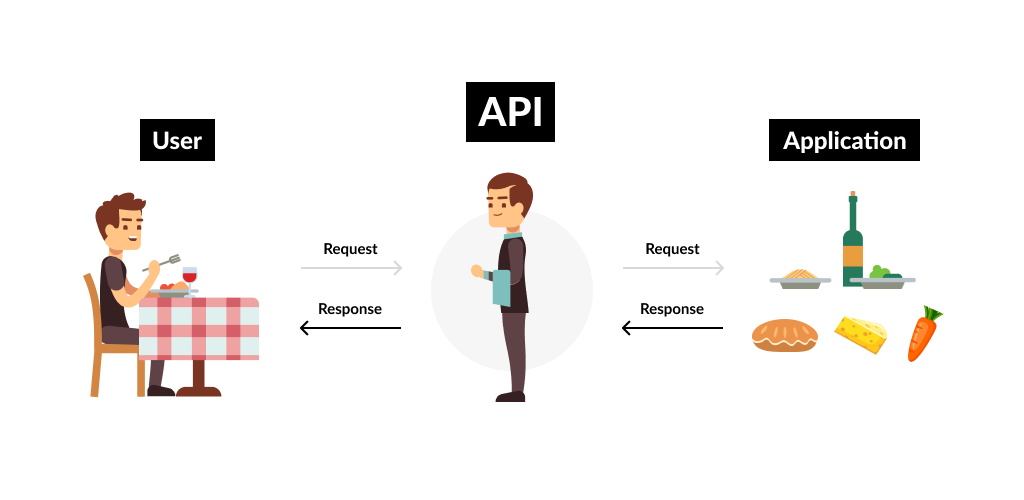
\includegraphics{images/api.png}
\caption{Interaksi melalui API}
\end{figure}
\end{frame}

\hypertarget{api-umum}{%
\section{API Umum}\label{api-umum}}

\begin{frame}{API Umum}
Secara umum untuk bisa menggunakan API di R minimal kita perlu
menginstall dua package berikut:

\begin{enumerate}
\tightlist
\item
  httr
\item
  jsonlite
\end{enumerate}
\end{frame}

\hypertarget{membuat-permintaan-request}{%
\subsection{Membuat permintaan
(request)}\label{membuat-permintaan-request}}

\begin{frame}[fragile]{Membuat permintaan (request)}
\begin{columns}[T]
\begin{column}{0.4\textwidth}
Secara umum setidaknya ada tiga hal yang bisa dilakukan oleh kita
(sebagai pengguna API), yaitu

\begin{enumerate}
\tightlist
\item
  GET() untuk mendapatakan data
\item
  POST() untuk mengirim data keserver
\item
  PUT()
\end{enumerate}

Coba gunakan \texttt{?httr} untuk melihat dokumentasi terkait dengan
semua yang bisa dilakukan menggunakan package ini.
\end{column}

\begin{column}{0.6\textwidth}
Contoh:

\begin{Shaded}
\begin{Highlighting}[]
\FunctionTok{library}\NormalTok{(httr)}
\FunctionTok{library}\NormalTok{(jsonlite)}

\NormalTok{github\_api }\OtherTok{\textless{}{-}} \ControlFlowTok{function}\NormalTok{(path) \{}
\NormalTok{  url }\OtherTok{\textless{}{-}} \FunctionTok{modify\_url}\NormalTok{(}
     \StringTok{"https://api.github.com"}\NormalTok{,}
     \AttributeTok{path =}\NormalTok{ path)}
  \FunctionTok{GET}\NormalTok{(url)}
\NormalTok{\}}

\NormalTok{what }\OtherTok{=} \StringTok{"commits"}
\NormalTok{resp }\OtherTok{\textless{}{-}} \FunctionTok{github\_api}\NormalTok{(}
   \FunctionTok{paste0}\NormalTok{(}
      \StringTok{"/repos/eppofahmi/belajaR/"}\NormalTok{, what))}
\end{Highlighting}
\end{Shaded}
\end{column}
\end{columns}
\end{frame}

\hypertarget{mengolah-data-yang-hasilkan}{%
\subsection{Mengolah data yang
hasilkan}\label{mengolah-data-yang-hasilkan}}

\begin{frame}[fragile]{Mengolah data yang hasilkan}
Data yang dihasilkan dari API biasanya berupa \texttt{json}. Untuk itu
kita bisa menggunakan fungsi \texttt{fromJSON()} dari \texttt{jsonlite}
untuk menjadikannya data frame atau list.

\begin{Shaded}
\begin{Highlighting}[]
\NormalTok{data }\OtherTok{=} \FunctionTok{fromJSON}\NormalTok{(}\FunctionTok{rawToChar}\NormalTok{(resp}\SpecialCharTok{$}\NormalTok{content))}
\end{Highlighting}
\end{Shaded}

Di R, biasanya kita mengolah data dalam format data frame. Hasil dari
API yang umumnya berupa json ada yang bisa langsung dikonversi menjadi
data frame, namun jika hal tersebut tidak bisa dilakukan maka kita perlu
mem-preprocessingnya terlebih dahulu.
\end{frame}

\hypertarget{api-twitter}{%
\section{Api Twitter}\label{api-twitter}}

\begin{frame}{Api Twitter}
Twitter merupakan salah satu media sosial yang paling banyak digunakan,
baik di Indonesia maupun di Dunia secara umum. Twitter juga memiliki
beberapa pilihan api yang bisa digunakan oleh publik baik secara gratis
maupun berbayar. \vspace{0.1in} Pilihan untuk menggunakan yang gratis
atau berbayar perlu disesuaikan dengan kebutuhan masing-masing. Selain
itu, Twitter juga menyediakan akses API untuk kebutuhan riset akademis
yang memiliki rentang pengambilan data lebih panjang dibanding yang
gratis namun bisa didapatkan secara gratis.
\end{frame}

\hypertarget{mendapatkan-api-twitter}{%
\subsection{Mendapatkan API Twitter}\label{mendapatkan-api-twitter}}

\begin{frame}{Mendapatkan API Twitter}
Untuk mendapatkan API Twitter kita perlu \textbf{mendaftar, membaca
petunjuk resminya, dan mengikuti prosedur} yang telah ditetapkan oleh
Twitter.

Prosesnya kurang lebih sebagai berikut:

\begin{enumerate}
\tightlist
\item
  Membuat akun Twitter (Jika belum punya)
\item
  Membuat aplikasi
  \href{https://developer.twitter.com/en/apply-for-access}{di sini}
\item
  Mendapatkan API Key, API Key Secret, Access Token, Access Token Secret
  dan Bearer Token
\item
  Menggunakan Key dari langkah ke-3 untuk mengambil data
\end{enumerate}
\end{frame}

\hypertarget{menggunakan-api-twitter}{%
\subsection{Menggunakan API Twitter}\label{menggunakan-api-twitter}}

\begin{frame}[fragile]{Menggunakan API Twitter}
Untuk bisa melihat tahapan mendapatakan Key API TWITTER bisa mengikuti
petunjuk dengan menjalankan skrip berikut:

\begin{Shaded}
\begin{Highlighting}[]
\CommentTok{\# uncomment untuk menginstall library}
\CommentTok{\# install.packages("rtweet")}

\FunctionTok{library}\NormalTok{(rtweet)}
\FunctionTok{vignette}\NormalTok{(}\StringTok{"auth"}\NormalTok{)}
\end{Highlighting}
\end{Shaded}
\end{frame}

\begin{frame}[fragile]{Setup Autentifikasi}
\protect\hypertarget{setup-autentifikasi}{}
\begin{Shaded}
\begin{Highlighting}[]
\FunctionTok{library}\NormalTok{(rtweet)}

\NormalTok{token }\OtherTok{\textless{}{-}} \FunctionTok{create\_token}\NormalTok{(}
  \AttributeTok{app =} \StringTok{"app"}\NormalTok{,}
  \AttributeTok{consumer\_key =} \StringTok{"consumer\_key"}\NormalTok{,}
  \AttributeTok{consumer\_secret =} \StringTok{"consumer\_secret"}\NormalTok{,}
  \AttributeTok{access\_token =} \StringTok{"access\_token"}\NormalTok{,}
  \AttributeTok{access\_secret =} \StringTok{"access\_secret"}\NormalTok{)}
\end{Highlighting}
\end{Shaded}
\end{frame}

\begin{frame}[fragile]{Pengambilan data}
\protect\hypertarget{pengambilan-data}{}
\begin{Shaded}
\begin{Highlighting}[]
\NormalTok{?rtweet}\SpecialCharTok{::}\NormalTok{search\_tweets}

\NormalTok{hasil }\OtherTok{=}\NormalTok{ rtweet}\SpecialCharTok{::}\FunctionTok{search\_tweets}\NormalTok{(}\AttributeTok{q =} \StringTok{"chelsea"}\NormalTok{, }
                              \AttributeTok{n =} \DecValTok{100}\NormalTok{, }
                              \AttributeTok{type =} \StringTok{"mixed"}\NormalTok{)}
\FunctionTok{glimpse}\NormalTok{(hasil)}
\end{Highlighting}
\end{Shaded}
\end{frame}

\hypertarget{mengolah-data-yang-di-dapat}{%
\subsection{Mengolah data yang di
dapat}\label{mengolah-data-yang-di-dapat}}

\begin{frame}{Mengolah data yang di dapat}
Untuk mengolah data Twitter, setidaknya ada dua hal yang bisa dijadikan
sebagai awalah yaitu:

\begin{enumerate}
\tightlist
\item
  Analisis user, yang bisa dilakukan menggunakan SNA
\item
  Analisis konten, yang bisa dilakukan menggunakan sentimen, topic
  modelling atau juga bisa menggunakan pendekatan network analisis.
\item
  Terdapat beberapa package yang bisa digunakan untuk mengambil
  sekaligus analisis network seperti twitteR, graphTweets, dan
  lain-lain.
\end{enumerate}
\end{frame}


\section[]{}
\frame{\small \frametitle{Table of Contents}
\tableofcontents}
\end{document}
